% !TeX root = ../Fundamental-Physics-B.tex
% 第 2.3 节：几种常见的力

\section{几种常见的力}

常见力的判断是受力分析的基础。本节讨论后续动力学问题中最常用的重力、弹性力、支持力、摩擦力，并结合叠放物块、板块系统和斜面体问题说明摩擦力的判定方法。

\subsection{重力、弹性力与支持力}

近地面处，重力通常写为
\[
    \boldsymbol G=m\boldsymbol g,
    \qquad
    G=mg,
\]
方向竖直向下。严格地说，重力与地球对物体的万有引力并不完全等同，但在本章基础动力学问题中通常采用近地面重力模型。

弹簧在弹性限度内满足胡克定律：
\[
    \boldsymbol F=-k\boldsymbol x,
    \qquad
    F=k|\Delta l|.
\]
其中 $k$ 为劲度系数，负号表示弹簧弹力总是指向恢复形变的方向。

支持力是接触面形变产生的弹性力，方向垂直接触面。支持力大小不能默认等于 $mg$，而应由平衡条件或动力学方程决定。只有在水平面静止且无其他竖直外力时，才有 $N=mg$。

\subsection{摩擦力}

摩擦力方向由接触面间的相对运动或相对运动趋势决定，而不是简单由物体相对于地面的运动方向决定。

静摩擦力满足
\[
    0\le \lvert f_s\rvert\le f_{s,\max}=\mu_sN.
\]
只有在临界滑动时，才有
\[
    \lvert f_s\rvert=\mu_sN.
\]
滑动摩擦力大小通常为
\[
    f_k=\mu_kN,
\]
方向与接触面间的相对滑动方向相反。

处理摩擦问题时，可按以下顺序判断：
\begin{enumerate}
    \item 先确定接触面和正压力 $N$；
    \item 判断是否已经发生相对滑动；
    \item 若未滑动，先假设静摩擦力方向，再由动力学方程求出所需 $f_s$；
    \item 检查是否满足 $|f_s|\le\mu_sN$；
    \item 若不满足，则说明发生滑动，改用 $f_k=\mu_kN$。
\end{enumerate}

\subsection{例题 2.2：叠放木块的临界相对运动}

\begin{figure}[htbp]
    \centering
    \IfFileExists{images/ex-2-2-original.png}{%
        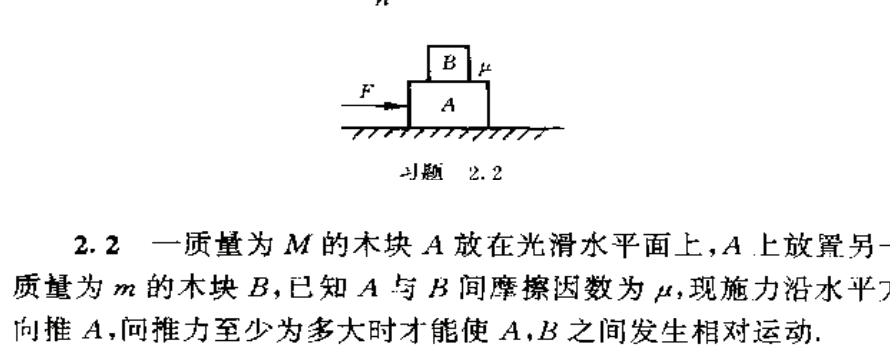
\includegraphics[width=0.72\textwidth]{images/ex-2-2-original.png}
    }{%
        \fbox{\parbox{0.72\textwidth}{\centering 原题图 2.2 预留位置：请将裁切后的图片命名为 \texttt{ex-2-2-original.png} 并放入 \texttt{images/} 目录。}}
    }
    \caption{习题 2.2 原题图}
\end{figure}

设下方木块 $A$ 的质量为 $M$，上方木块 $B$ 的质量为 $m$。水平面光滑，只有 $A$、$B$ 之间存在摩擦，摩擦因数为 $\mu$。若两者不发生相对运动，则它们具有共同加速度
\[
    a=\frac{F}{M+m}.
\]
上方木块 $B$ 的水平方向受力只有静摩擦力，因此所需静摩擦力为
\[
    f_s=ma=\frac{mF}{M+m}.
\]
不发生相对运动要求
\[
    f_s\le \mu mg.
\]
于是
\[
    \frac{mF}{M+m}\le \mu mg.
\]
因此临界推力为
\[
    \boxed{F_{临界}=\mu(M+m)g}.
\]
当 $F$ 大于该值时，所需静摩擦力超过最大静摩擦力，$A$、$B$ 之间发生相对运动。

\begin{center}
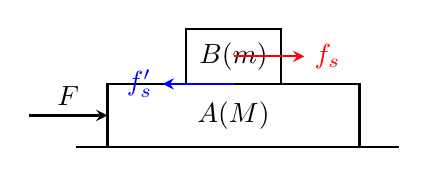
\begin{tikzpicture}[scale=1.0,>=stealth]
    \draw[thick] (0,0) rectangle (3.2,0.8);
    \draw[thick] (1.0,0.8) rectangle (2.2,1.5);
    \node at (1.6,0.4) {$A(M)$};
    \node at (1.6,1.15) {$B(m)$};
    \draw[thick] (-0.4,0) -- (3.7,0);
    \draw[->,thick] (-1.0,0.4) -- (0,0.4) node[midway,above] {$F$};
    \draw[->,thick,red] (1.6,1.15) -- (2.5,1.15) node[right] {$f_s$};
    \draw[->,thick,blue] (1.6,0.8) -- (0.7,0.8) node[left] {$f_s'$};
\end{tikzpicture}
\end{center}

本题易错点是把静摩擦力一开始就写成 $\mu mg$。事实上，静摩擦力先由共同运动所需的加速度决定，只有临界状态才达到最大值。

\subsection{例题 2.3：板与物体共同加速及抽板条件}

\begin{figure}[htbp]
    \centering
    \IfFileExists{images/ex-2-3-original.png}{%
        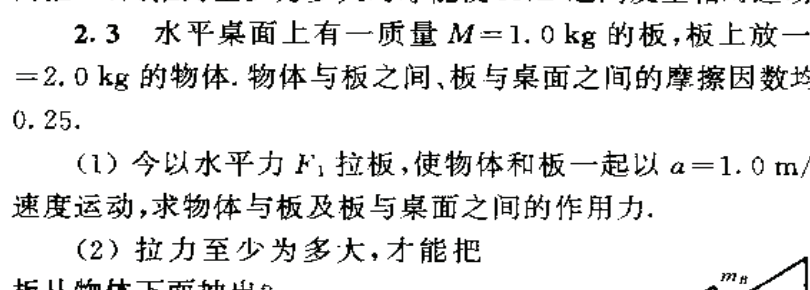
\includegraphics[width=0.82\textwidth]{images/ex-2-3-original.png}
    }{%
        \fbox{\parbox{0.82\textwidth}{\centering 习题 2.3 原题图预留位置：请将裁切后的图片命名为 \texttt{ex-2-3-original.png} 并放入 \texttt{images/} 目录。}}
    }
    \caption{习题 2.3 原题图}
\end{figure}

已知板质量 $M=1.0\,\mathrm{kg}$，物体质量 $m=2.0\,\mathrm{kg}$，物体与板之间、板与桌面之间的摩擦因数均为 $\mu=0.25$。

\subsubsection*{（1）共同以 $a=1.0\,\mathrm{m/s^2}$ 加速}

物体 $m$ 的水平方向受力只有来自板的静摩擦力，因此
\[
    f_1=ma=2.0\times1.0=2.0\,\mathrm{N}.
\]
物体与板之间的正压力为
\[
    N_1=mg=2.0g.
\]
取 $g=9.8\,\mathrm{m/s^2}$，则
\[
    N_1=19.6\,\mathrm{N},\qquad
    f_{1,\max}=\mu N_1=4.9\,\mathrm{N}.
\]
由于所需静摩擦力 $2.0\,\mathrm{N}$ 小于最大静摩擦力，物体与板可保持相对静止。

板与桌面之间的正压力为
\[
    N_2=(M+m)g=3.0g=29.4\,\mathrm{N}.
\]
板相对桌面滑动时，桌面对板的滑动摩擦力大小为
\[
    f_2=\mu N_2=0.25\times29.4=7.35\,\mathrm{N}.
\]
因此，物体与板之间的作用力包括正压力 $19.6\,\mathrm{N}$ 和摩擦力 $2.0\,\mathrm{N}$；板与桌面之间的作用力包括正压力 $29.4\,\mathrm{N}$ 和摩擦力 $7.35\,\mathrm{N}$。

\subsubsection*{（2）刚要把板从物体下抽出}

刚要发生相对滑动时，物体与板之间的静摩擦力达到最大：
\[
    f_{1,\max}=\mu mg.
\]
物体能够随板共同运动的最大加速度为
\[
    a_{\max}=\frac{f_{1,\max}}{m}=\mu g.
\]
把板和物体作为整体，在临界状态下有
\[
    F-\mu(M+m)g=(M+m)a_{\max}.
\]
代入 $a_{\max}=\mu g$，得
\[
    F_{\min}=2\mu(M+m)g.
\]
数值上
\[
    \boxed{F_{\min}=2\times0.25\times3.0\times9.8=14.7\,\mathrm{N}}.
\]

\subsection{例题 2.4：斜面体保持静止的摩擦条件}

\begin{figure}[htbp]
    \centering
    \IfFileExists{images/ex-2-4-original.png}{%
        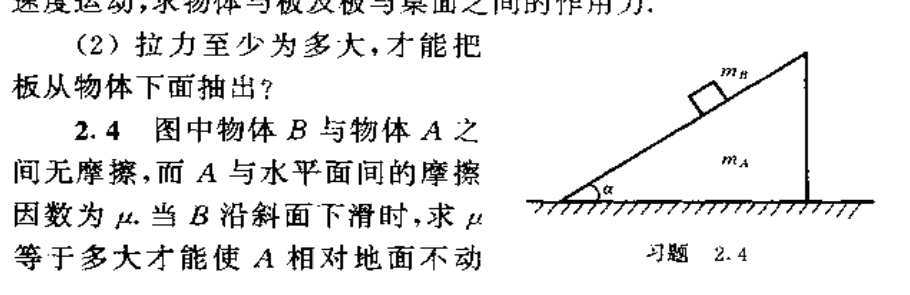
\includegraphics[width=0.82\textwidth]{images/ex-2-4-original.png}
    }{%
        \fbox{\parbox{0.82\textwidth}{\centering 原题图 2.4 预留位置：请将裁切后的图片命名为 \texttt{ex-2-4-original.png} 并放入 \texttt{images/} 目录。}}
    }
    \caption{习题 2.4 原题图}
\end{figure}

物体 $B$ 与斜面体 $A$ 之间无摩擦，$A$ 与水平地面之间的摩擦因数为 $\mu$。设 $B$ 正沿斜面下滑，要求 $A$ 相对地面不动。

由于 $A$ 不动，可把斜面看作固定斜面分析 $B$。垂直斜面方向无加速度，因此
\[
    N=m_Bg\cos\alpha.
\]
这里 $N$ 是斜面 $A$ 对物体 $B$ 的支持力。由牛顿第三定律，$B$ 对 $A$ 的压力大小也为 $N$，方向垂直斜面向右下方。其水平分量为
\[
    N\sin\alpha=m_Bg\sin\alpha\cos\alpha,
\]
竖直向下分量为
\[
    N\cos\alpha=m_Bg\cos^2\alpha.
\]

对斜面体 $A$，地面对它的支持力为
\[
    N_0=m_Ag+N\cos\alpha
       =m_Ag+m_Bg\cos^2\alpha.
\]
为使 $A$ 不动，地面对 $A$ 的静摩擦力必须平衡 $B$ 对 $A$ 的水平推力：
\[
    f_s=N\sin\alpha=m_Bg\sin\alpha\cos\alpha.
\]
静摩擦力不能超过最大静摩擦力：
\[
    f_s\le \mu N_0.
\]
因此
\[
    m_Bg\sin\alpha\cos\alpha
    \le
    \mu\left(m_Ag+m_Bg\cos^2\alpha\right),
\]
化简得
\[
    \boxed{
    \mu \ge
    \frac{m_B\sin\alpha\cos\alpha}
    {m_A+m_B\cos^2\alpha}
    }.
\]

\begin{center}
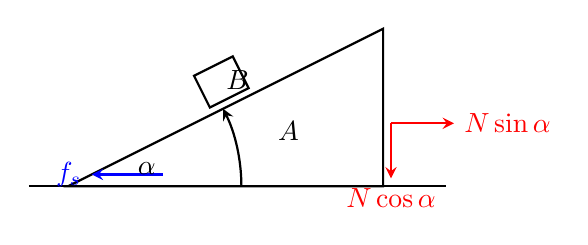
\begin{tikzpicture}[scale=1.0,>=stealth]
    \coordinate (O) at (0,0);
    \coordinate (R) at (4,0);
    \coordinate (T) at (4,2);
    \draw[thick] (O) -- (R) -- (T) -- cycle;
    \draw[thick] (-0.5,0) -- (4.8,0);
    \node at (2.8,0.7) {$A$};
    \draw[rotate around={26.565:(1.8,1.0)},thick] (1.8,1.0) rectangle (2.35,1.45);
    \node at (2.15,1.35) {$B$};
    \draw[->,thick,red] (4.1,0.8) -- (4.9,0.8) node[right] {$N\sin\alpha$};
    \draw[->,thick,red] (4.1,0.8) -- (4.1,0.1) node[below] {$N\cos\alpha$};
    \draw[->,thick,blue] (1.2,0.15) -- (0.3,0.15) node[left] {$f_s$};
    \draw[->,thick] (2.2,0) arc (0:26.565:2.2);
    \node at (1.0,0.22) {$\alpha$};
\end{tikzpicture}
\end{center}
